\subsection{SVM amb RBF kernel}

En aquesta secció s'explicarà el desenvolupament del mètode de Màquines de Vectos de Suport (SVM en anglès) usant el kernel \textit{Radial Basis Function} per tal de tenir un model no lineal. 

Aquest mètode necessita dos paràmetres, $C$ amb l'objectiu de reduir el sobreajust i $\sigma$. Per tal d'establir la millor combinació d'ambdós paràmetres s'ha usat \textit{5-fold Cross-Validation} en el test d'entrenament tal com s'ha explicat a la secció~\ref{prepros}. La decisió d'usar \textit{5-fold} i no un altre mètode més precís (ja sigui una $k$ més gran o repetir el procés $x$ vegades) ha estat perquè el temps d'execució d'aquest procés ja era bastant elevat. Per realitzar aquest mètode s'ha escalat els valors d'ambdós conjunts de dades usant la funció \verb|scale()| de R.

S'ha decidit usar el següent conjunt de valors de $C$ i de $\sigma$. 
\[C: 0.01, 0.1, 1 , 10, 100, 1000\]
\[\sigma: 0.03125, 0.0625, 0.125, 0.25, 0.5, 1, 2, 4\]

\begin{table}[H]
\centering
\begin{adjustbox}{max width=\textwidth}
\begin{tabular}{|r|r|r|r|r|r|}
  \hline
C & sigma & Accuracy & Kappa & AccuracySD & KappaSD \\ 
  \hline
  0.01 & 0.0312 & 0.3740 & 0.3482 & 0.0051 & 0.0053 \\ 
  0.01 & 0.0625 & 0.4634 & 0.4415 & 0.0044 & 0.0046 \\ 
  0.10 & 2.0000 & 0.0953 & 0.0570 & 0.0056 & 0.0058 \\ 
  0.10 & 4.0000 & 0.0466 & 0.0062 & 0.0010 & 0.0010 \\ 
  1.00 & 0.1250 & 0.9521 & 0.9501 & 0.0026 & 0.0027 \\ 
  1.00 & 0.2500 & 0.9609 & 0.9593 & 0.0023 & 0.0023 \\ 
  10.00 & 0.0312 & 0.9510 & 0.9490 & 0.0022 & 0.0023 \\ 
  10.00 & 4.0000 & 0.5496 & 0.5311 & 0.0057 & 0.0059 \\ 
  \textbf{100.00} & \textbf{0.1250} & \textbf{0.9680} & \textbf{0.9668} & \textbf{0.0012} & \textbf{0.0012} \\ 
  100.00 & 2.0000 & 0.8129 & 0.8054 & 0.0082 & 0.0086 \\ 
  100.00 & 4.0000 & 0.5496 & 0.5311 & 0.0057 & 0.0059 \\ 
  1000.00 & 1.0000 & 0.9296 & 0.9268 & 0.0030 & 0.0031 \\ 
  1000.00 & 4.0000 & 0.5496 & 0.5311 & 0.0057 & 0.0059 \\ 
   \hline
\end{tabular}
\end{adjustbox}
\caption{Subconjunt dels resultats de \textit{5-fold Cross-Validation} usant $C$ i $\sigma$}
\label{cvTaula}
\end{table}

Com es pot observar en la taula~\ref{cvTaula} els millors paràmetres pel model són: $C = 100$ i $\sigma = 0.1250$ que s'obté un encert del 96.8\% en \textit{Cross-Validation}. En la figura~\ref{fig:c_validation} es pot observar l'evolució de l'encert en la predicció en funció dels diferents valors de $C$ i $\sigma$.

\begin{figure}[H]
    \centering
    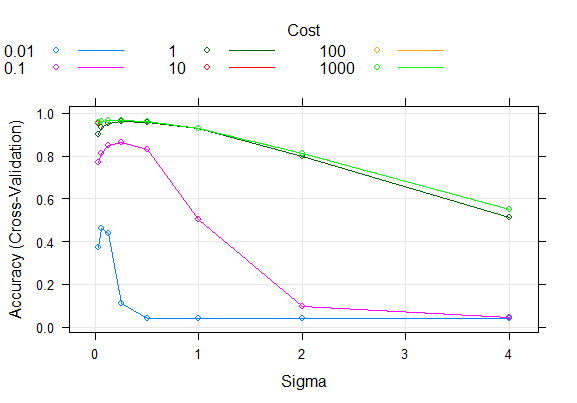
\includegraphics[width=0.8\textwidth]{img/SVMRBF_CV.png}
    \caption{Evolució de la predicció de Cross-Validation en funció de $C$ i $\sigma$}
    \label{fig:c_validation}
\end{figure} 

El model aconsegueix un 97.54\% d'encert en el conjunt de dades de prova.